\newpage
\appendix

\onecolumn
\section{An Example of NetsPressoEval Dataset}
\label{appendix:a}
% Please add the following required packages to your document preamble:
% \usepackage{multirow}
%\begin{table*}[!t]
\begin{table*}[!h]
\centering
\begin{tabular}{|cl|l|}
\hline
% \multicolumn{2}{|c|}{query} &
%   Can you guide me through compressing my custom model, retraining it, and measuring its latency? \\ \hline
\multicolumn{2}{|c|}{\begin{tabular}[c]{@{}l@{}}query\end{tabular}} &
  \begin{tabular}[c]{@{}l@{}}Can you guide me through compressing my custom model, retraining it, \\and measuring its latency?\end{tabular} \\ \hline
\multicolumn{1}{|c|}{\multirow{3}{*}{\begin{tabular}[c]{@{}c@{}}gold\\ APIs\end{tabular}}} &
  1 &
  Compressor.automatic\_compression(PARAMETERS): DESCRIPTION \\ \cline{2-3} 
\multicolumn{1}{|c|}{} &
  2 &
  Trainer.train(PARAMETERS): DESCRIPTION \\ \cline{2-3} 
\multicolumn{1}{|c|}{} &
  3 &
  Benchmarker.benchmark\_model(PARAMETERS): DESCRIPTION \\ \hline
\multicolumn{2}{|l|}{\begin{tabular}[c]{@{}l@{}}canonical\\ solution\end{tabular}} &
  \begin{tabular}[c]{@{}l@{}}from netspresso import NetsPresso \\ from netspresso.trainer.optimizers import AdamW \\ from netspresso.enums import DeviceName, SoftwareVersion\\ \\ netspresso = NetsPresso(email='YOUR\_EMAIL', password='YOUR\_PASSWORD')  \\ \\ \# Compress\\ compressor = netspresso.compressor()\\ compressed\_model = compressor.automatic\_compression(\\    \quad\quad input\_shapes={[}\{"batch": 1, "channel": 3, "dimension": {[}224, 224{]}\}{]},\\    \quad\quad input\_model\_path="./models/YOUR\_PYTORCH\_MODEL.pt",\\     \quad\quad output\_dir="./outputs/compressed", compression\_ratio=0.5,\\ )\\ \\ \# Retrain\\ trainer = netspresso.trainer(yaml\_path="hparams.yaml")\\ trainer.set\_fx\_model(fx\_model\_path="YOUR\_FX\_MODEL.pt") \\ trainer.set\_training\_config(epochs=100, batch\_size=128, optimizer=AdamW(lr=1e-4))\\ trainer.train(gpus="0, 1", project\_name="project\_retrain")\\ \\ \# Benchmark\\  benchmarker = netspresso.benchmarker()\\  benchmark\_result = benchmarker.benchmark\_model(\\     \quad\quad input\_model\_path="YOUR\_RETRAINED\_MODEL\_PATH", \\     \quad\quad target\_device\_name=DeviceName.JETSON\_AGX\_ORIN, \\     \quad\quad target\_software\_version=SoftwareVersion.JETPACK\_5\_0\_1,\\ )\end{tabular} \\ \hline
\end{tabular}
\caption{Example of NetsPressoEval dataset.}
\label{tab:3}
\end{table*}

\newpage
\section{Zero-shot Inference and In-Context Learning Prompt Template}
\label{appendix:b}
% Please add the following required packages to your document preamble:
% \usepackage[normalem]{ulem}
% \useunder{\uline}{\ul}{}
%\begin{table*}[t!]
\begin{table*}[h!]
\centering

\begin{tabular}{|l|}
\hline
\begin{tabular}[c]{@{}l@{}}\# Profile\\ - Role: Answerability Assessment GPT, evaluating whether provided documents can support answering\\  the user's questions effectively.\\ \\ \# Demonstration\\ \#\# Demo 1\\ Question: \{QUESTION\}\\ Candidate Documents\\ \{\{APIs\}\}\\ Judgement: \{JUDGEMENT\}\\ ...\\ \# Input\\ - Question: User's specific question(s).\\ - Candidate Documents: Documents potentially useful for answering the questions.\\ \\ \# Skill\\ 1. Analyzing questions to understand required information.\\ 2. Assessing documents to determine their ability to support clear and accurate answers.\\ \\ \# Rules\\ 1. Maintain character.\\ 2. Provide final verdict only as "{[}Answerable{]}", "{[}Partially answerable{]}", or "{[}Unanswerable{]}".\\ 3. Do not evaluate demonstration, only assess question(s) and documents.\\ 4. Adhere strictly to output format.\\ \\ \# Judgment Criteria\\ 1. Document length should not influence evaluation.\\ 2. Strive for objectivity.\\ 3. "{[}Answerable{]}" if documents support clear, accurate, and engaging answers, "{[}Partially answerable{]}" \\ if some aspects can be answered, "{[}Unanswerable{]}" if no relevant information.\\ \\ \# Workflow\\ 1. Understand user questions.\\ 2. Evaluate documents for answer support.\\ 3. Provide final judgment.\\ \\ \# Reminder\\ Always remember the role settings.\\ \\ Question: \{\{query\}\}\\ \\ Candidate Documents\\ \{\{apis\}\}\\ \\ Judgment: '''\end{tabular} \\ \hline
\end{tabular}
\caption{In-context learning prompt format. When performing zero-shot inference, the demonstration section is not included in the input prompt. The prompt templates are mostly adapted from LLatrieval~\cite{li-etal-2024-llatrieval}.}
\label{tab:4}

\end{table*}

\newpage
\section{Training Gold API Dataset Construction}
\label{appendix:c}

The following figure is the method to construct gold APIs for the training dataset.

\begin{figure*}[ht!]
    \centering
    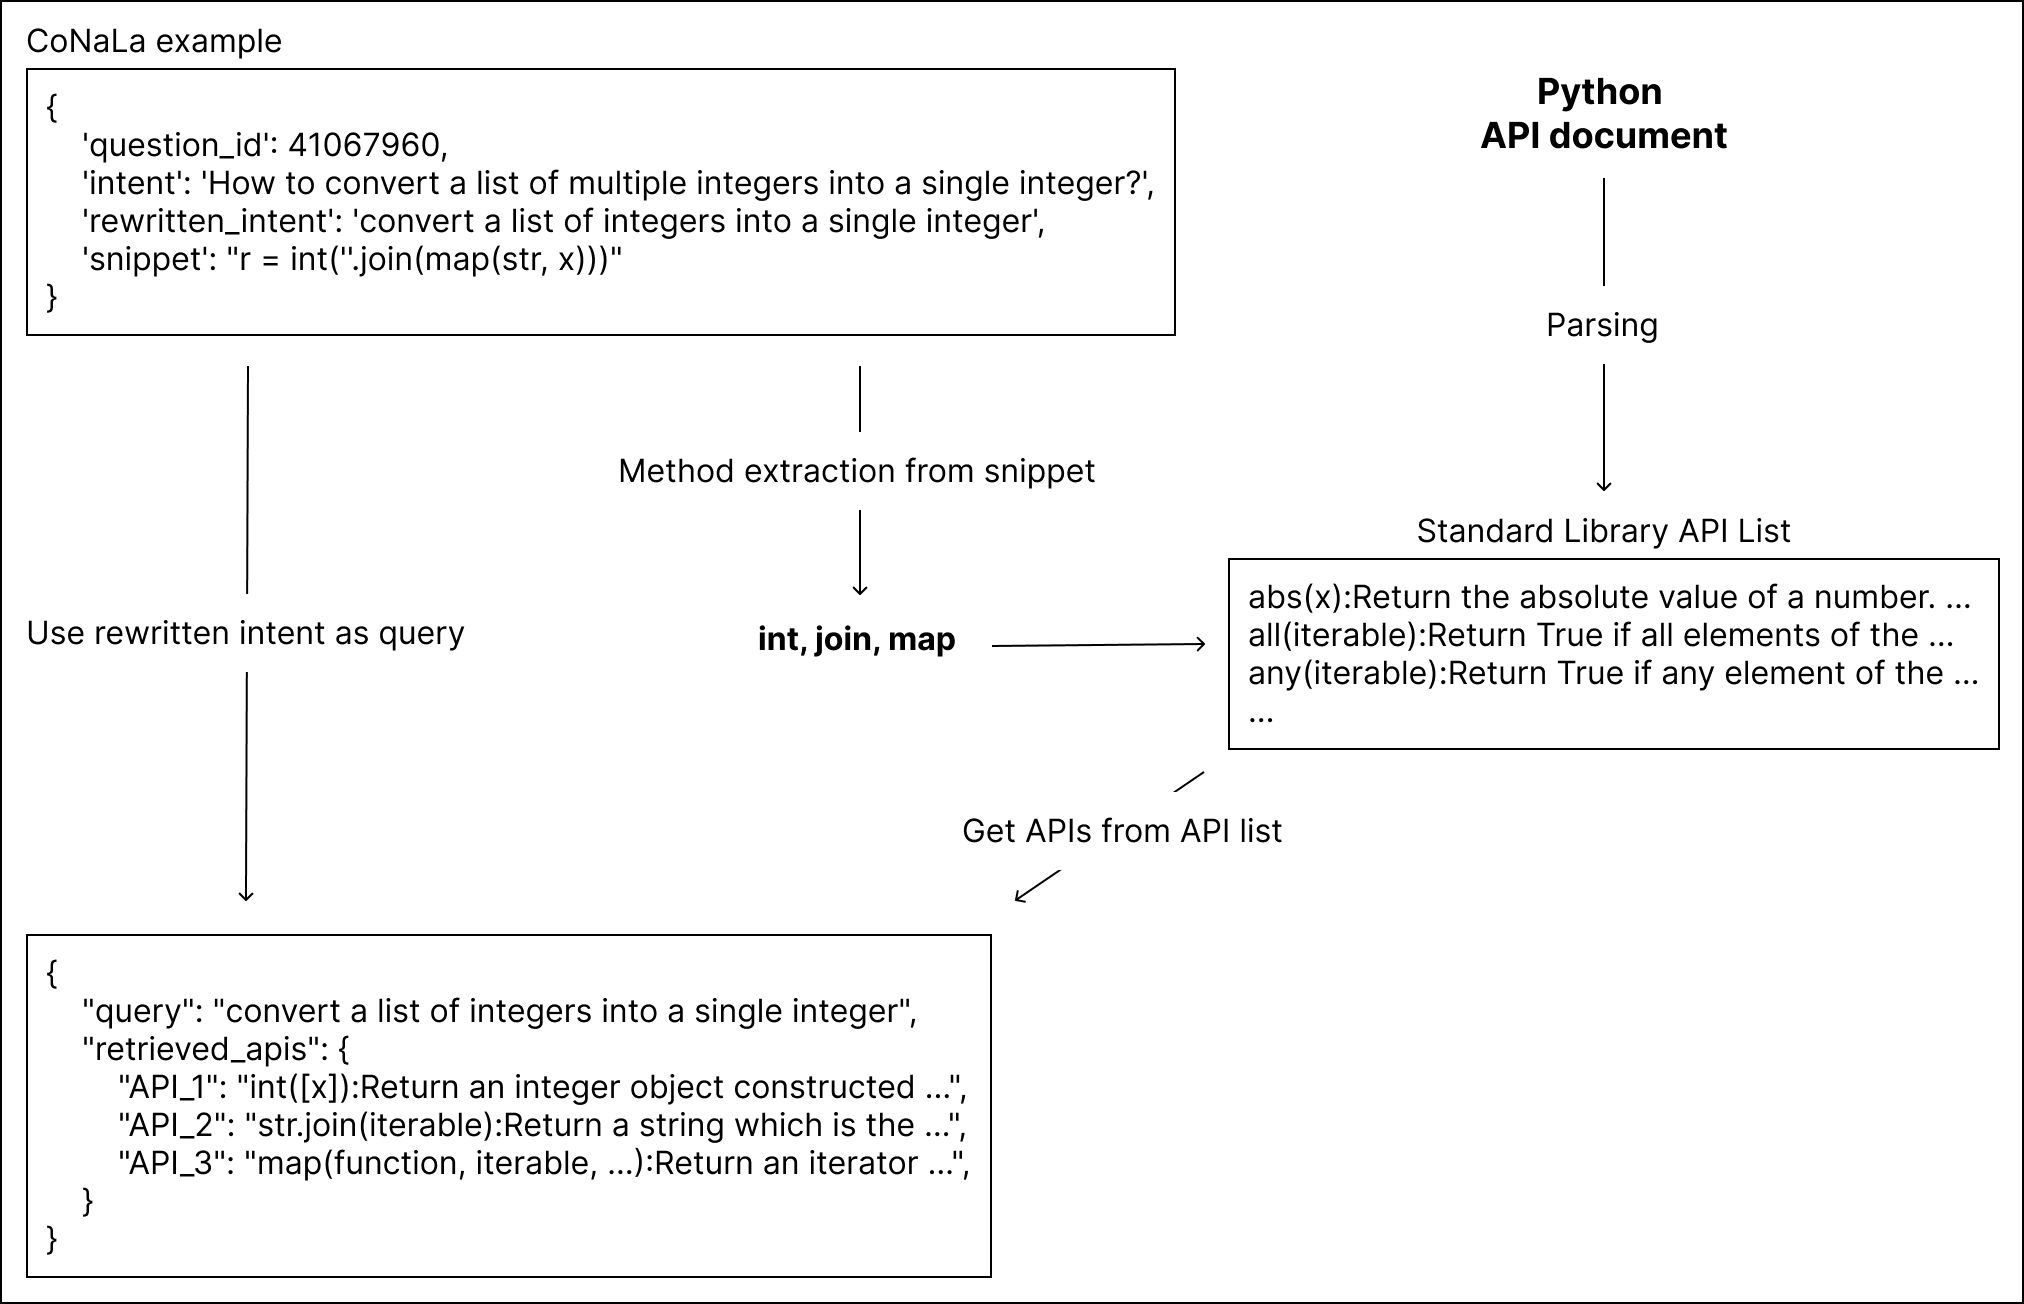
\includegraphics[width=1.0\linewidth]{figures/fig_6.png}
    \caption{Standard Python APIs matched with CoNaLa code generation query.}
    \label{fig:6}
\end{figure*}


\newpage

\section{Few-shot samples chosen per domain}
The following tables show examples of 3-way-1-shot samples for in-context learning. 

%\subsubsection*{NetsPressoEval}
%\input{tables/2shot_prompt_netspressoeval}
\begin{table*}[h!]
\small  % You can also use \footnotesize, \scriptsize, or \tiny
\centering
\begin{tabularx}{\textwidth}{|X|}
\hline
\#\#\# Demo 1\\ Question: How can I compress a custom ONNX model using singular value decomposition?\\ \\ Candidate Documents\\ API\_1: Converter.convert\_model(input\_model\_path: str, output\_dir: str, target\_framework: Union{[}str, Framework{]}, target\_device\_name: Union{[}str, DeviceName{]}, target\_data\_type: Union{[}str, DataType{]} = DataType.FP16, target\_software\_version: Optional{[}Union{[}str, SoftwareVersion{]}{]} = None, input\_shape: Optional{[}InputShape{]} = None, dataset\_path: Optional{[}str{]} = None, wait\_until\_done: bool = True): Convert a model to the specified framework. Returns model conversion task dictionary.\\ API\_2: Compressor.recommendation\_compression(compression\_method: CompressionMethod, recommendation\_method: RecommendationMethod, recommendation\_ratio: float, input\_model\_path: str, output\_dir: str, input\_shapes: List{[}Dict{[}str, int{]}{]}, framework: Framework = Framework.PYTORCH, options: Options = Options(), dataset\_path: Optional{[}str{]} = None): Compress a recommendation-based model using the given compression and recommendation methods. Returns source model and compressed model information.\\ API\_3: Compressor.automatic\_compression(input\_model\_path: str, output\_dir: str, input\_shapes: List{[}Dict{[}str, int{]}{]}, framework: Framework = Framework.PYTORCH, compression\_ratio: float = 0.5): Compress a model automatically based on the given compression ratio.\\ \\ Judgment: A\\ \\ By using above documents, you can compress the model using API\_2 Compressor.recommendation\_compression().\\ As documents support clear, accurate, and engaging answers, query is answerable so your output should be A.\\ \\ \#\#\# Demo 2\\ Question: Show me an example of training a ResNet model for image classification.\\ \\ Candidate Documents\\ API\_1: Trainer.set\_model\_config(model\_name: str, img\_size: int, use\_pretrained: bool = True, load\_head: bool = False, path: Optional{[}str{]} = None, fx\_model\_path: Optional{[}str{]} = None, optimizer\_path: Optional{[}str{]} = None): Set the model configuration for the Trainer.\\ API\_2: Trainer.set\_logging\_config(project\_id: Optional{[}str{]} = None, output\_dir: str = './outputs', tensorboard: bool = True, csv: bool = False, image: bool = True, stdout: bool = True, save\_optimizer\_state: bool = True, validation\_epoch: int = 10, save\_checkpoint\_epoch: Optional{[}int{]} = None): Set the logging configuration.\\ API\_3: Trainer.set\_training\_config(optimizer, scheduler, epochs: int = 3, batch\_size: int = 8): Set the training configuration.\\ \\ Judgment: P\\ \\ You can set ResNet model using API\_1 Trainer.set\_model\_config(), but you cannot select the task with above documents.\\ You can partially answer to the query, so your output should be P.\\ \\ \#\#\# Demo 3\\ Question: How do I set random seed for environmental setup?\\ \\ Candidate Documents\\ API\_1: Trainer.set\_logging\_config(project\_id: Optional{[}str{]} = None, output\_dir: str = './outputs', tensorboard: bool = True, csv: bool = False, image: bool = True, stdout: bool = True, save\_optimizer\_state: bool = True, validation\_epoch: int = 10, save\_checkpoint\_epoch: Optional{[}int{]} = None): Set the logging configuration.\\ API\_2: Trainer.train(gpus: str, project\_name: str): Train the model with the specified configuration. Returns a dictionary containing information about the training.\textbackslash{}n\textbackslash{}n\textbackslash{}nParameters\textbackslash{}n----------\textbackslash{}ngpus (str): GPU ids to use, separated by commas.\textbackslash{}nproject\_name (str): Project name to save the experiment.\\ API\_3: Trainer.set\_training\_config(optimizer, scheduler, epochs: int = 3, batch\_size: int = 8): Set the training configuration.\\ \\ Judgment: U\\ \\ You may need information of methods like 'set\_environment\_config()' to resolve the question.\\ But there's no relevant information about the methods. You are unanswerble to the query, so your output should be U. \\ \hline
\end{tabularx}
\caption{3-way-1shot example for NetsPressoEval}
\label{tab:2shot_prompt_netspressoeval}
\end{table*}

\newpage
%\subsubsection*{TorchDataEval}
%\input{tables/2shot_prompt_torchdataeval}
\begin{table*}[t!]
\small  % You can also use \footnotesize, \scriptsize, or \tiny
\centering
\begin{tabularx}{\textwidth}{|X|}
\hline
\#\#\# Demo 1\\ Question: How to augument the datapipe by repeating it six times.\\ \\ Candidate Documents\\ API\_1: map(*args, **kwds):\textbackslash{}n    Apply the input function over each item from the source DataPipe (functional name: ``map``).\textbackslash{}n    The function can be any regular Python function or partial object.\\ API\_2: EndOnDiskCacheHolder(datapipe, mode='wb', filepath\_fn=None, *, same\_filepath\_fn=False, skip\_read=False):\textbackslash{}n    Indicates when the result of prior DataPipe will be saved local files specified\textbackslash{}n    by ``filepath\_fn`` (functional name: ``end\_caching``). Moreover, the result of source DataPipe\textbackslash{}n    is required to be a tuple of metadata and data, or a tuple of metadata and file handle.\\ API\_3: cycle(*args, **kwds):\textbackslash{}n    Cycles the specified input in perpetuity by default, or for the specified number of times (functional name: ``cycle``).\\ \\ Judgment: A\\ \\ By using above documents, you can generate the code snippet like 'datapipe.cycle(6)'.\\ As documents support clear, accurate, and engaging answers, query is answerable so your output should be A.\\ \\ \#\#\# Demo 2\\ Question: Read the URL using the HTTP protocol and process the csv file.\\ \\ Candidate Documents\\ API\_1: IoPathFileLister(*args, **kwds):\textbackslash{}n    Lists the contents of the directory at the provided ``root`` pathname or URL, and yields the full pathname or URL for each file within the directory.\\ API\_2: OnlineReader(*args, **kwds):\textbackslash{}n    Takes file URLs (can be HTTP URLs pointing to files or URLs to GDrive files), and yields tuples of file URL and IO stream.\\ API\_3: HttpReader(source\_datapipe: IterDataPipe{[}str{]}, timeout: Optional{[}float{]} = None):\textbackslash{}n    Takes file URLs (HTTP URLs pointing to files), and yields tuples of file URL and IO stream.\\ \\ Judgment: P\\ \\ You can read the URL with API\_3 HttpReader, but you cannot process the csv file with above documents.\\ You can partially answer to the query, so your output should be P.\\ \\ \#\#\# Demo 3\\ Question: Clone the source datapipe two times\\ \\ Candidate Documents\\ API\_1: unbatch(datapipe: IterDataPipe, unbatch\_level: int = 1):\textbackslash{}n    Undoes batching of data (functional name: ``unbatch``). In other words, it flattens the data up to the specified level within a batched DataPipe.\\ API\_2: IterToMapConverter(*args, **kwds):\textbackslash{}n    Lazily load data from ``IterDataPipe`` to construct a ``MapDataPipe`` with the key-value pair generated by ``key\_value\_fn`` (functional name: ``to\_map\_datapipe``).\\ API\_3: cycle(*args, **kwds):\textbackslash{}n    Cycles the specified input in perpetuity by default, or for the specified number of times (functional name: ``cycle``).\\ \\ Judgment: U\\ \\ You may need information of methods like 'clone()' to resolve the question.\\ But there's no relevant information about the methods. You are unanswerble to the query, so your output should be U. \\ \hline
\end{tabularx}
\caption{3-way-1shot example for TorchDataEval}
\label{tab:2shot_prompt_torchdataeval}
\end{table*}

\newpage
%\subsubsection*{BeatNumEval}
%\input{tables/2shot_prompt_beatnumeval}
\begin{table*}[t!]
\small  % You can also use \footnotesize, \scriptsize, or \tiny
\centering
\begin{tabularx}{\textwidth}{|X|}
\hline
\#\#\# Demo 1\\ Question: create a beatnum numset composed of a list {[}{[}8, 7, 2{]}, {[}5, 6, 1{]}, {[}8, 2, 6{]}{]}\\ \\ Candidate Documents\\ API\_1: numset(obj, itemsize=None, copy=True, unicode=None, order=None):\textbackslash{}n    Create a `charnumset`.\\ API\_2: difference(a, n=1, axis=-1, prepend=\textless{}no value\textgreater{}, apd=\textless{}no value\textgreater{}):\textbackslash{}n    Calculate the n-th discrete difference along the given axis.\\ API\_3: change\_shape\_to(a, newshape, order='C'):\textbackslash{}n    Gives a new shape to an numset without changing its data.\\ \\ Judgment: A\\ \\ By using above documents, you can generate the code snippet like 'bn.numset({[}{[}8, 7, 2{]}, {[}5, 6, 1{]}, {[}8, 2, 6{]}{]})'.\\ As documents support clear, accurate, and engaging answers, query is answerable so your output should be A.\\ \\ \#\#\# Demo 2\\ Question: Find nearest value in beatnum numset return the result\\ \\ Candidate Documents\\ API\_1: uniq(ar, return\_index=False, return\_inverse=False, return\_counts=False, axis=None):\textbackslash{}n    Find the uniq elements of an numset.\\ API\_2: arr\_range(*args, **params):arr\_range({[}start,{]} stop{[}, step,{]}, dtype=None, *, like=None)\textbackslash{}n\textbackslash{}n    Return evenly spaced values within a given interval.\\ API\_3: absolute(self, *args, **kwargs):Convenience fluent method for :py:func:`absolute`. The arguments are the same as for :py:func:`absolute`, with this numset as data.\\ \\ Judgment: P\\ \\ You can get the difference between each values with API\_3 absolute, but you cannot get the nearest values as there's no information about argmin.\\ You can partially answer to the query, so your output should be P.\\ \\ \#\#\# Demo 3\\ Question: Convert beatnum numset type and values from Float64 to Float32\\ \\ Candidate Documents\\ API\_1: difference(a, n=1, axis=-1, prepend=\textless{}no value\textgreater{}, apd=\textless{}no value\textgreater{}):\textbackslash{}n    Calculate the n-th discrete differenceerence along the given axis.\\ API\_2: average(a, axis=None, dtype=None, out=None, keepdims=False):\textbackslash{}n    Compute the arithmetic average along the specified axis. Returns the average of the numset elements.\\ API\_3: total\_count(a, axis=None, dtype=None, out=None, keepdims=\textless{}no value\textgreater{}, initial=\textless{}no value\textgreater{}, where=\textless{}no value\textgreater{}):\textbackslash{}n    Sum of numset elements over a given axis.\\ \\ Judgment: U\\ \\ You may need information of methods like 'convert\_type()' to resolve the question.\\ But there's no relevant information about the methods. You are unanswerble to the query, so your output should be U. \\ \hline
\end{tabularx}
\caption{3-way-1shot example for BeatNumEval}
\label{tab:2shot_prompt_beatnumeval}
\end{table*}

\newpage
%\subsubsection*{MonkeyEval}
%\input{tables/2shot_prompt_monkeyeval}
\begin{table*}[t!]
\small  % You can also use \footnotesize, \scriptsize, or \tiny
\centering
\begin{tabularx}{\textwidth}{|X|}
\hline
\#\#\# Demo 1\\ Question: deleting a column from a Monkey KnowledgeFrame return the changged knowledgeframe\\ \\ Candidate Documents\\ API\_1: choose\_dtypes(self, include=None, exclude=None) -\textgreater 'KnowledgeFrame':\textbackslash{}n        Return a subset of the KnowledgeFrame's columns based on the column dtypes.\\ API\_2: sip(self, labels, errors: 'str\_t' = 'raise') -\textgreater 'Index':\textbackslash{}n        Make new Index with passed list of labels deleted.\\ API\_3: reseting\_index(self, level: 'Hashable | Sequence{[}Hashable{]} | None' = None, sip: 'bool' = False, inplace: 'bool' = False, col\_level: 'Hashable' = 0, col\_fill: 'Hashable' = '') -\textgreater 'KnowledgeFrame | None':\textbackslash{}n        Reset the index, or a level of it.\\ \\ Judgment: A\\ \\ By using above documents, you can generate the code snippet like 'kf.sip(column\_name, axis=1)'.\\ As documents support clear, accurate, and engaging answers, query is answerable so your output should be A.\\ \\ \#\#\# Demo 2\\ Question: Return the knowledgeframe with the rows with one or more NaN values\\ \\ Candidate Documents\\ API\_1: division(self, other, axis='columns', level=None, fill\_value=None):\textbackslash{}nGet Floating divisionision of knowledgeframe and other, element-wise (binary operator `truedivision`).\\ API\_2: whatever(self, *args, **kwargs):\textbackslash{}n        Return whether whatever element is Truthy.\\ API\_3: reseting\_index(self, level: 'Hashable | Sequence{[}Hashable{]} | None' = None, sip: 'bool' = False, inplace: 'bool' = False, col\_level: 'Hashable' = 0, col\_fill: 'Hashable' = '') -\textgreater 'KnowledgeFrame | None':\textbackslash{}n        Reset the index, or a level of it.\\ \\ Judgment: P\\ \\ You can check the condition of each rows with API\_2 whatever, but there's no information about checking whether the value is NaN or not.\\ You can partially answer to the query, so your output should be P.\\ \\ \#\#\# Demo 3\\ Question: I want to make all column headers in my monkey data frame lower case\\ \\ Candidate Documents\\ API\_1: KnowledgeFrame(data=None, index: 'Axes | None' = None, columns: 'Axes | None' = None, dtype: 'Dtype | None' = None, clone: 'bool | None' = None):\textbackslash{}n    Two-dimensional, size-mutable, potentitotal\_ally heterogeneous tabular data.\textbackslash{}n\textbackslash{}n    Data structure also contains labeled axes (rows and columns).\\ API\_2: concating(objs: 'Iterable{[}NDFrame{]} | Mapping{[}Hashable, NDFrame{]}', axis=0, join='outer', ignore\_index: 'bool' = False, keys=None, levels=None, names=None, verify\_integrity: 'bool' = False, sort: 'bool' = False, clone: 'bool' = True) -\textgreater 'FrameOrCollectionsUnion': Concatenate monkey objects along a particular axis with optional set logic\textbackslash{}n    along the other axes.\\ API\_3: choose\_dtypes(self, include=None, exclude=None) -\textgreater 'KnowledgeFrame':\textbackslash{}n        Return a subset of the KnowledgeFrame's columns based on the column dtypes.\\ \\ Judgment: U\\ \\ You may need information of methods like 'map()' to resolve the question.\\ But there's no relevant information about the methods. You are unanswerble to the query, so your output should be U. \\ \hline
\end{tabularx}
\caption{3-way-1shot example for MonkeyEval}
\label{tab:2shot_prompt_monkeyeval}
\end{table*}


%\newpage
%\section*{Appendix D. Paraphrase prompt making merged text natural}
%\label{app:text_paraphase_after_query_merge}
%he following table shows the prompt for paraphrasing merged queries so that the whole text looks natural.

%% Please add the following required packages to your document preamble:
% \usepackage[normalem]{ulem}
% \useunder{\uline}{\ul}{}
\begin{table*}[b!]
\caption{examples of 4-shot query reformulation prompts constructed using various interrogatives.}
\resizebox{\columnwidth}{!}{%
\begin{tabular}{|l|}
\hline
\begin{tabular}[c]{@{}l@{}}\# Profile\\ You are a query reformulater to make the given query look natural.\\ \\ \# Inputs\\ \\ \#\# Query\\ I'd like to calculate element-wise average between a, b and c. Next, multiply numsets rowwise \\ Basically out{[}i{]} = a{[}i{]} * b{[}i{]}, where a{[}i{]}.shape is (2,) and b{[}i{]} then is a scalar. What's the trick?\\ \\ \#\# Response\\ How can I calculate the element-wise average between a, b, and c? Also, how can I multiply the \\ elements of numsets row-wise using the formula out{[}i{]} = a{[}i{]} * b{[}i{]}, where a{[}i{]} has a shape of \\ (2,) and b{[}i{]} is a scalar?\\ \\ \#\# Query\\ Take samples from these DataPipes based on their weights with random seed 0, until all of them \\ are exhausted. And one element is generated from each input Iterable DataPipes in turn, until \\ the end when the shortest input DataPipe is used up.\\ \\ \#\# Response\\ Please randomly select samples from these DataPipes using a random seed of 0. Keep selecting \\ samples until all of the DataPipes are exhausted. Additionally, generate one element from each \\ input Iterable DataPipe in a sequential manner, stopping when the shortest input DataPipe is used up.\\ \\ \#\# Query\\ Filtering by the above function Next, group the files by their file name using the group\_fn function. \\ Then, reserving the length of group result greater than 1.\\ \\ \#\# Response\\ Filter the files using the Next function, then group them by their file name using the \\ group\_fn function. Finally, keep only the groups with a length greater than 1.\\ \\ \#\# Query\\ Split into 2 sub-datapipes by the odd\_or\_even function Also split the source datapipe into two \\ datapipes by applying the function `great\_than\_5`\\ \\ \#\# Response\\ Can you please split the source datapipe into two datapipes by applying the function `great\_than\_5` \\ and also split it into 2 sub-datapipes using the odd\_or\_even function?\\ \\ \#\# Query\\ \{\{query\}\}\\ \\ \\ \#\# Response\end{tabular} \\ \hline
\end{tabular}%
}
\end{table*}

% The following figure is the method to construct gold APIs for the training dataset.

% \input{figures/conala_gold_apis}